
\begin{frame}
  \frametitle{Context}
  \begin{itemize}
  \item Time-indexed model more efficient {\small (relatively stronger relaxation)}
    \pause
    \vfill
  \item But:
    \begin{itemize}
    \item  model size depends on planning horizon 
      
      $\longrightarrow $ for large planning horizon event-based model can be more
      efficient (RCPSP:~{\color{gray!50!black!70}\it [Koné et al.,
        2011]} )
      \vfill
      \pause
    \item  if only non-integer solutions
      
      $\longrightarrow$ time-indexed model can lead to
      infeasible/sub-optimal solution
      (CECSP:~{\color{gray!50!black!70}\it [Nattaf et al., 2015]} )
    \end{itemize}
  \end{itemize}
  \vfill
  \pause
  {\bf Goal: Tightened Event-based models (2 exists)} 
\end{frame}
\begin{frame}{Start/End formulation}
  {\small \it Adaptation of a model for the RCPSP {\color{gray!50!black!50} \it [Koné et al., 2011]}}
  \vfill
  \begin{block}{Variables}
    \begin{itemize}
    \item  $t_e$ represents the event (start or end time)
      \pause
      \vspace{0.3cm}
    \item $x_{ie}=\left\{
        \begin{array}{ll}
          1 & \text{if $i$ starts at event $e$ (time $t_e$)}\\
          0 & \text{otherwise}
        \end{array}
      \right.
      $
      \pause
      \vspace{0.3cm}
    \item $y_{ie}=\left\{
        \begin{array}{ll}
          1 & \text{if $i$ ends at event $e$ (time $t_e$)}\\
          0 & \text{otherwise}
        \end{array}
      \right.
      $
      \vspace{0.3cm}
      \pause
    \item $B_{ie}$: resource quantity consumed by $i$ in $\inter[t_e][t_{e+1}]$
      \vspace{0.3cm}
      \pause
    \item $W_{ie}$: energy brought to $i$ in $\inter[t_e][t_{e+1}]$   
    \end{itemize}
  \end{block}
\end{frame}


\begin{frame}{Event-based model}
  \vfill
  \begin{itemize}
  \item Start/End model have stronger relaxations than the On/Off
    model ( $z_{ie} = \sum_{f=1}^e x_{if} - \sum_{f=1}^e y_{if}$)
    \pause
    \vfill
  \item But: On/Off model has less variables than Start/End model
    \pause
    and  better performances  
    \vfill
    \pause
  \item Study of the On-Off formulation
    \vfill
    \pause
  \item Collaboration with Tam{\'a}s Kis 
  \end{itemize} 
  \vfill
\end{frame}

\begin{frame}{Event-based model}
  \vfill 
  {\bf On/Off Model}
  {\footnotesize
    \begin{eqnarray*}
      \textcolor<1>{blue!80!black!80}{t_e \le t_{e+1} }&
                                                         \textcolor<1>{blue!80!black!80}{ \forall e}\\[2mm]
      \pause
      \textcolor<2>{blue!80!black!80}{r_iz_{ie}\le t_e
      } & \textcolor<2>{blue!80!black!80}{\forall e, i
          }\\[2mm] 
      \textcolor<2>{blue!80!black!80}{t_e \le
      lst_i(z_{ie}-z_{ie-1})+(1-(z_{ie}-z_{ie-1}))D_{max} }&
                                                             \textcolor<2>{blue!80!black!80}{ \forall e,i}\\[2mm]
      \pause
      \textcolor<3>{blue!80!black!80}{ 
      eet_i(z_{ie-1}-z_{ie})\le t_e} & \textcolor<3>{blue!80!black!80}{
                                       \forall e, i }\\[2mm]
      \textcolor<3>{blue!80!black!80}{t_e \le
      d_i(z_{ie-1}-z_{ie})+(1-(z_{ie-1}-z_{ie}))D_{max}}&
                                                            \textcolor<3>{blue!80!black!80}{\forall e, i }\\[2mm]
      \pause
      \textcolor<4>{blue!80!black!80}{ \sum_{e \in {\cal E}}
      z_{ie} \ge 1}& \textcolor<4>{blue!80!black!80}{\forall i
                     } \\[2mm]
      \textcolor<4>{blue!80!black!80}{\sum_{e'=1}^{e}
      z_{ie'} \le e(1-(z_{ie}-z_{ie-1})) }& \textcolor<4>{blue!80!black!80}{
                                            \forall e,i}\\[2mm]
      \textcolor<4>{blue!80!black!80}{\sum_{e'=e}^{2n}
      z_{ie'} \le (2n-e)(1+(z_{ie}-z_{ie-1})) }&
                                                 \textcolor<4>{blue!80!black!80}{\forall e,i}
    \end{eqnarray*}}
  \vfill
\end{frame}


\subsection{Valid inequalities}
\begin{frame}
  \frametitle{Maximum separation between events}
  \begin{itemize}
  \item {\bf Goal: } upper bound on the value of $t_{e+1}-t_{e}$
    \vspace{0.3cm}
  \item<2-> Time window of each task start and/or end time
    \vspace{0.3cm}
  \item<6-> An event must occur in each of these time windows
    \vspace{0.3cm}
  \item<11-> two consecutive events in the union of two consecutive time windows
  \end{itemize}
  \vfill
  \onslide<3->{
    \begin{center} 
      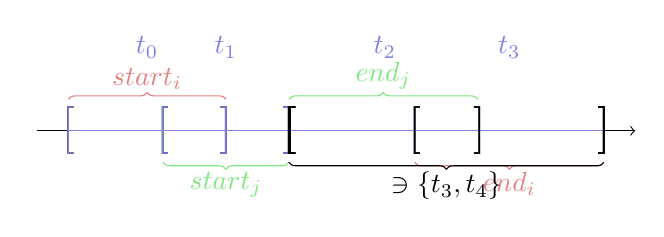
\begin{tikzpicture}
        [decoration={brace},scale=0.4]
        \node (O) at (0,0) {}; 
        \draw[->] (0,0) -- (19,0);

        \onslide<4-5>{
          \path (1,0) node[color=red!80!black!50] {\LARGE [} --
          +(0:5cm)node[color=red!80!black!50] {\LARGE ]};
          \path[green!80!black!50](4,0) node {\LARGE [} -- +(0:4cm)
          node {\LARGE ]};
          \path[green!80!black!50] (8.05,0) node {\LARGE [}  --
          +(0:6cm) node {\LARGE ]}  ;
          \path (12,0) node[color=red!80!black!50] {\LARGE [} --
          +(0:6cm) node[color=red!80!black!50] {\LARGE ]} ; 
        }
        
        \onslide<4>{
          \draw [decorate,color=red!80!black!50] (1,1) -- +(0:5cm)
          node[midway,above]{$start_i$}; 
          \draw [decorate,color=red!80!black!50] (18,-1) -- +(0:-6cm)
          node[midway,below] {$end_i$};
        }
        
        \onslide<5>{
          \draw [decorate,green!80!black!50] (8,-1) -- +(0:-4cm)
          node[midway,below] {$start_j$};
          \draw [decorate,green!80!black!50] (8,1) -- +(0:6cm)
          node[midway,above] {$end_j$};
        }
        
        \onslide<6-9>{
          \path (1,0) node {\LARGE [} --
          +(0:5cm)node {\LARGE ]};
          \path(4,0) node {\LARGE [} -- +(0:4cm)
          node {\LARGE ]};
          \path (8.05,0) node {\LARGE [}  --
          +(0:6cm) node {\LARGE ]}  ;
          \path (12,0) node {\LARGE [} --
          +(0:6cm) node {\LARGE ]} ; 
        }

        \onslide<6>{
          \path[blue!80!black!50,draw] (1,0) node {\LARGE [} -- +(0:5cm)node
          {\LARGE ]} node[midway,above=0.8cm] {$t_0$};
        }
        \onslide<7>  {
          \path[blue!80!black!50,draw](4,0) node {\LARGE [} --
          +(0:4cm) node {\LARGE ]} node[midway,above=0.8cm] {$t_1$}; 
        }
        
        \onslide<8>{   
          \path[blue!80!black!50,draw] (8.05,0) node {\LARGE [}  --
          +(0:6cm) node {\LARGE ]}  node[midway,above=0.8cm] {$t_2$};
        }
        
        \onslide<9>{
          \path[blue!80!black!50,draw] (12,0) node {\LARGE [} --
          +(0:6cm) node {\LARGE ]} node[midway,above=0.8cm] {$t_3$};
        }
        
        \onslide<10>{
          \path (12,0) node {\LARGE [}  --
          +(0:6cm) node {\LARGE ]}  ;
          \path (8.05,0) node {\LARGE [}  --
          +(0:6cm) node {\LARGE ]}  ;
        }
        \onslide<11>{
          \path (12,0) --
          +(0:6cm) node {\LARGE ]}  ;
          \path (8.05,0) node {\LARGE [}  --
          +(0:6cm)  ;
        }
        
        \onslide<12>{
          \path (8,0) node {\LARGE [} --
          +(0:10cm) node {\LARGE ]}  ;
          \draw [decorate] (18,-1) -- +(0:-10cm)
          node[midway,below] {$\ni \{t_3,t_{4}\}$};
        }
      \end{tikzpicture}
    \end{center}
  }
\end{frame}

\begin{frame}
  \frametitle{Maximum separation between events}
  \begin{itemize}
  \item Order the time-window intervals according to:
    \[ [a,b] \le [c,d]
      \Leftrightarrow a < c \lor \left( a=c \land b \le d\right)\]
    \vfill
    \pause
  \item Then we have:
    \[t_{e+1}-t_e  \le   |tw_e \cup tw_{e+1}|    \]
    \pause
    \begin{flushright}
      \textcolor{black!70}{\scriptsize in fact: $t_{e+1}-t_e  \le
        \overline{tw_e \cup tw_{e+1}} - \underline{tw_e \cup tw_{e+1}}
        $}
    \end{flushright}
    \pause
    \vfill
  \item We can use it as:
    \begin{itemize}
      \vspace{0.2cm}
    \item additional constraints of the model
    \item an upper bound on $t_{e+1}-t_e$ in any constraints using a worst one
    \end{itemize}
  \end{itemize}
\end{frame}

\begin{frame}
  \frametitle{Maximum time for an event}
  \begin{itemize}
  \item {\bf Goal: } upper bound on the value of $t_{e}$
    \vspace{0.4cm}
  \item<2-> upper bound of each task start and/or end time
    \vspace{0.4cm}
  \item<5-> an event must occur before each of these upper bounds
    \vspace{0.4cm}
  \end{itemize}
  \vfill
  \onslide<3->{
    \begin{center} 
      \begin{tikzpicture}
        [decoration={brace},scale=0.4]
        \node (O) at (0,0) {}; 
        
        \draw[->] (0,0) -- (19,0);
        \onslide<3>{
          \draw (1,0) node {\LARGE [} -- +(0:5cm)node {\LARGE ]}; 
          
          \draw(4,0) node {\LARGE [} -- +(0:4cm) node {\LARGE ]} ;
          
          \draw (8.05,0) node {\LARGE [}  --
          +(0:6cm) node {\LARGE ]}  ;
          \draw (12,0) node {\LARGE [} --
          +(0:6cm) node {\LARGE ]}  ;}
        \onslide<4>{
          
          \draw (1,0) node {} -- +(0:5cm)node {\LARGE ]}; 
          
          \draw(4,0) node {} -- +(0:4cm) node {\LARGE ]} ;
          
          \draw (8.05,0) node {}  --
          +(0:6cm) node {\LARGE ]}  ;
          \draw (12,0) node {} --
          +(0:6cm) node {\LARGE ]}  ;}
        \onslide<5>{
          \draw[color=blue!80!black!50] (0,0) node {} -- +(0:6cm)node {\LARGE ]}
          node[left,above=0.8cm] {$t_0$}; 
          \draw (8,0) node {\LARGE ]} ;
          \draw (8.05,0) node {}  -- +(0:6cm) node {\LARGE ]}  ;
          \draw (12,0) node {} -- +(0:6cm) node {\LARGE ]}  ;}
        
        \onslide<6>{
          \draw (6,0) node  {\LARGE ]}; 
          \draw[color=blue!80!black!50](0,0) -- (8,0) node {\LARGE ]} node[left,above=0.8cm] {$t_1$};
          \draw (8.05,0) node {}  --  +(0:6cm) node {\LARGE ]}  ;
          \draw (12,0) node {} --  +(0:6cm) node {\LARGE ]}  ;}
        
        \onslide<7>{
          \draw (6,0) node {\LARGE ]}; 
          \draw (8,0) node {\LARGE ]} ;
          \draw[color=blue!80!black!50] (0,0) node {}  -- (14,0) node {\LARGE ]} node[left,above=0.8cm] {$t_2$} ;
          \draw (18,0)node {\LARGE ]}  ;}
        
        \onslide<8>{
          \draw (6,0) node {\LARGE ]}; 
          \draw(8,0) node {\LARGE ]} ;
          \draw (14,0) node {\LARGE ]}  ;
          \draw[color=blue!80!black!50] (0,0) node {} -- (18,0) node {\LARGE ]}
          node[left,above=0.8cm] {$t_3$};} 
        
      \end{tikzpicture}
    \end{center}
  }
\end{frame}


\begin{frame}
  \frametitle{Maximum time for an event}
  \begin{itemize}
  \item Order the time-window interval upper bounds ${\cal UP}$ in
    increasing order 
    \vfill
    \pause
  \item Then we have:
    \[t_e \le  {\cal UP}_e\]
    \vfill
    \pause
  \item We can use it as:
    \begin{itemize}
      \vspace{0.2cm}
    \item additional constraints of the model
    \item an upper bound on $t_{e+1}-t_e$ in any constraints using a worst one
    \end{itemize}
  \end{itemize}
\end{frame}

\subsection{Polyhedral results}


\begin{frame}
  \frametitle{$Z_i$-polyhedron}
  \vspace{0.5cm}
  \onslide<1->{$\rightarrow$ Minimal set of inequalities defining the
    {\it ``$Z_i$-polyhedron''}.}
  \vspace{0.6cm}
  \onslide<2-> {  \begin{block}{$Z_i$-polyhedron}
      form of $z_i \in \{0,1\}^{|{\cal E}|}$ solution? \hspace{2.5cm}
      {\scriptsize (${\cal E}=$event set)}}
    \vspace{0.4cm}

    \onslide<4->{$\Rightarrow$ vector with consecutive-one property  and at least
      one $1$
      \begin{center}
        {\small e.g. $(0,0,1,1,1,0),\ (1,1,1,0,0,0),\ \dots$}
      \end{center}}
    \onslide<5->{     
      \[Z_i= conv\{z_i \in \{0,1\}^{|{\cal E}|} | z_i \text{ of the
          form } (0^*\, 1\, 1^*\, 0^*)\} \] }
    \vspace{-0.2cm}
  \end{block}
  \onslide<3->{\textcolor{black!70}{ \small\[z_{ie}=\left\{
          \begin{array}{ll}
            1 & \text{if task $i$ is in process between $t_e$ and $t_{e+1}$}\\
            0 & \text{otherwise}
          \end{array}
        \right.
      \]}}
\end{frame}

\begin{frame}
  \frametitle{Non-preemptive inequalities}

  \begin{itemize}
  \item $ z_{ie}-z_{if}+z_{ig} \le 1$ enforces
    $z_{if}$ to be $1$ for all $e<f<g$ s.t. $z_{ie}=z_{ig}=1$ 
  \end{itemize}
  \pause
  \vspace{0.4cm}
  \begin{block}{Non-preemptive inequalities }
    Generalization of constraints $ z_{ie}-z_{if}+z_{ig} \le 1$ to
    every subset of events of odd cardinality (GNP).
  \end{block}
  \pause
  \vspace{0.4cm}
  \[ZP_i=\{ z_i \in [0,1]^{\cal E} | z_i\text{ satisfies
      GNP inequalities and } \eqref{eq1}\}\] 
  \begin{equation}
    \text{ with }  \sum_{e \in \cal E} z_{ie} \ge 1 \quad \forall i \in \cal A  
    \label{eq1}  
  \end{equation}
  \pause
  \vspace{0.4cm}
  \begin{block}{Theorem}
    \[ZP_i=Z_i\]
  \end{block}
  \vspace{0.5cm}
\end{frame}


\begin{frame}
  \frametitle{Computational experience}
  \begin{itemize}
    \vfill
  \item Intel Core i7-4770 processor with 4 cores and 8Go of RAM
    \vfill
  \item OS: 64-bit Ubuntu 12.04
    \vfill
  \item MILP resolution: CPLEX 12.6 with 1 thread  
    \vfill
  \item Special separation procedure for non-preemptive cuts ($O(n^2)$)
    for node with depth less than 10
    \vfill
  \item time limit: 1000 seconds
    \vfill
  \end{itemize}
\end{frame}

\pgfplotstableread[row sep=\\,col sep=&]{
  tasks & Default & Int. & Time & Preem. & I+T+P \\
  20    & 164.14 & 182.2 & 167.3 & 330.9 & 154  \\
  25     & 635.4 & 727.3 & 629.5 & 822.4 & 389.9 \\
  30    & 968  & 851 & 961.4 & 914.8 & 813.8\\
}\mydata

\begin{frame}
  \frametitle{Time comparison for the CECSP}
  \begin{itemize}
  \item Instances of {\it [Nattaf et al.,2015]}
  \item 10 instances of 20, 25 and 30 tasks
  \end{itemize}

  \vspace{0.2cm}
  \begin{center}\begin{tikzpicture}
      \begin{axis}[ enlarge x limits=0.25,
        ybar,
        bar width=.4cm,  
        legend style={at={(0.5,1)},
          anchor=north,legend columns=-1},
        width=\textwidth,
        height=.6\textwidth,
        symbolic x coords={20,25,30},
        xtick=data,
        ymin=0,ymax=1100,
        ylabel={\small time (s)},
        xlabel={\small $\#tasks$}]
        \addplot table[x=tasks,y=Default]{\mydata};
        \addplot table[x=tasks,y=Int.]{\mydata};
        \addplot table[x=tasks,y=Time]{\mydata};
        \addplot table[x=tasks,y=Preem.]{\mydata};
        \addplot table[x=tasks,y=I+T+P]{\mydata};
        \legend{Default ,Int. , Time , Preem. ,I+T+P}
      \end{axis}
    \end{tikzpicture}
  \end{center}
\end{frame}

\pgfplotstableread[row sep=\\,col sep=&]{
  tasks & Default & Int. & Time & Preem. & I+T+P \\
  20    & 90.9 & 90.9 & 90.9 & 72.7 & 90.9\\
  25     &55.6 & 55.6 & 88.9 & 44.4 & 77.8\\
  30    & 10 & 20& 20& 10 &60\\
}\mydat
\begin{frame}
  \frametitle{Solved instances comparison for the CECSP}
  \begin{itemize}
  \item Instances of {\color{gray!50!black!70}\it [Nattaf et al., 2015]}
  \item 10 instances of 20, 25 and 30 tasks
  \end{itemize}

  \vspace{0.2cm}
  \begin{center}\begin{tikzpicture}
      \begin{axis}[ enlarge x limits=0.25,
        ybar,
        bar width=.4cm,  
        legend style={at={(0.5,1)},
          anchor=north,legend columns=-1},
        width=\textwidth,
        height=.6\textwidth,
        symbolic x coords={20,25,30},
        xtick=data,
        ymin=0,ymax=110,
        ylabel={\small $\%solved$},
        xlabel={\small $\#tasks$}]
        \addplot table[x=tasks,y=Default]{\mydat};
        \addplot table[x=tasks,y=Int.]{\mydat};
        \addplot table[x=tasks,y=Time]{\mydat};
        \addplot table[x=tasks,y=Preem.]{\mydat};
        \addplot table[x=tasks,y=I+T+P]{\mydat};
        \legend{Default ,Int. , Time , Preem. ,I+T+P}
      \end{axis}
    \end{tikzpicture}
  \end{center}
\end{frame}

\pgfplotstableread[row sep=\\,col sep=&]{
  tasks & Default & Int. &  Preem. & I+P \\
  30    & 34.8 & 30.3& 30.3& 33.1\\
}\mydat
  \begin{frame}
    \frametitle{Time comparison for the RCPSP}
    \begin{itemize}
    \item Instances of {\color{gray!50!black!70} \it [Koné et al., 2011]}
    \item 480 instances of 30 tasks
    \end{itemize}

    \vspace{0.3cm}
    \begin{center}
      \begin{tikzpicture}
      \begin{axis}[ enlarge x limits=0.25,
        ybar,
        bar width=.8cm,  
        legend style={at={(0.5,1)},
          anchor=north,legend columns=-1},
        width=0.8\textwidth,
        height=.55\textwidth,
        symbolic x coords={30},
        xtick=data,
        ymin=0,ymax=50,
        ylabel={\small $time (s)$},
        xlabel={\small $\#tasks$}]
        \addplot table[x=tasks,y=Default]{\mydat};
        \addplot table[x=tasks,y=Int.]{\mydat};
        \addplot table[x=tasks,y=Preem.]{\mydat};
        \addplot table[x=tasks,y=I+P]{\mydat};
        \legend{Default ,Int. , Time , Preem. ,I+T+P}
      \end{axis}
    \end{tikzpicture}
    \end{center}
  \end{frame}
